A \Figref{grafico-resultados} apresenta a comparação entre os resultados de
simulação e os obtidos experimentalmente no \gls{tecolab}, ambos avaliados sobre
a mesma curva de referência. Como métrica de desempenho adotou-se o \gls{rmse},
definido na \Eqref{rmse}, calculado sobre o erro de seguimento da temperatura
relativa do sensor 2.

O sistema simulado apresentou $\mathrm{RMSE} = 1{,}3567\,^\circ\mathrm{C}$,
enquanto o ensaio experimental resultou em $\mathrm{RMSE} =
2{,}2956\,^\circ\mathrm{C}$. Em ambos os casos, a estratégia composta por
\gls{pd} e \gls{ff} acompanhou a referência ao longo do regime transitório em
rampa e do regime permanente em $40\,^\circ\mathrm{C}$, recuperando-se após a
perturbação aplicada aos 10 minutos. O incremento de aproximadamente
$0{,}94\,^\circ\mathrm{C}$ no \gls{rmse} experimental em relação ao simulado
indica boa aderência entre o modelo e o sistema físico, ainda que com desempenho
inferior ao previsto em simulação.

\begin{figure}[H]
\centering
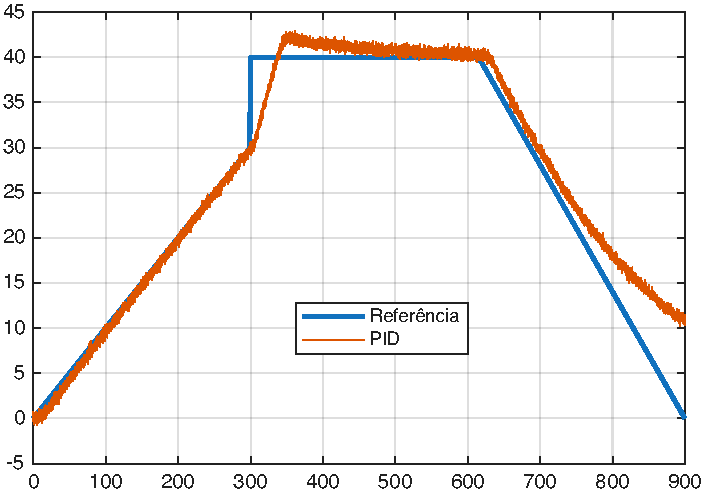
\includegraphics[width=1\linewidth]{images/Resultados.pdf}
\caption{Comparação entre os resultados simulado e experimental quanto ao
seguimento da curva de referência de temperatura relativa do sensor 2.}
\figlabel{grafico-resultados}
\end{figure}